Die Produktfunktionen beschreiben jede einzelne Funktion des Produkts mittels Anwendungsfalldiagrammen und Anwendungsfalltabellen.
\\\\
In  Tabelle~\autoref{fig:akteur-tabelle} werden alle auftretenden Akteure beschrieben.


\begin{figure}[h]
	\centering

	\begin{tabularx}{\textwidth}{ p{.2\textwidth} | p{.4\textwidth} | X }
		\textbf{Akteur} & \textbf{Beschreibung} & \textbf{Verwendet in Anwendungsszenario} \\ \hline
		unregistrierteR NutzerIn & Nicht angemeldeter NutzerIn. Kann nur Kompositionen einsehen & APP-2, APP-3, WEB-6
		\\ \hline NutzerIn & Angemeldeter NutzerIn. Nutzt den SWARM Composer & APP-1, APP-2, APP-3, APP-4, WEB-4, WEB-5, WEB-6
		\\ \hline AdministratorIn & Nutzt und verwaltet den SWARM-Composer & APP-1, APP-2, APP-3, APP-4, WEB-1, WEB-2, WEB-3, WEB-4, WEB-5, WEB-6
	\end{tabularx}

	\caption{Beschreibung der Akteure}
	\label{fig:akteur-tabelle}
\end{figure}


%%%%%%%%%%%%%%%
%% Anwendungsfall 1 %%
%%%%%%%%%%%%%%%
\newpage

\section{Anwendungsfalldiagramm - App}

\begin{figure}[h]
	\centering	
	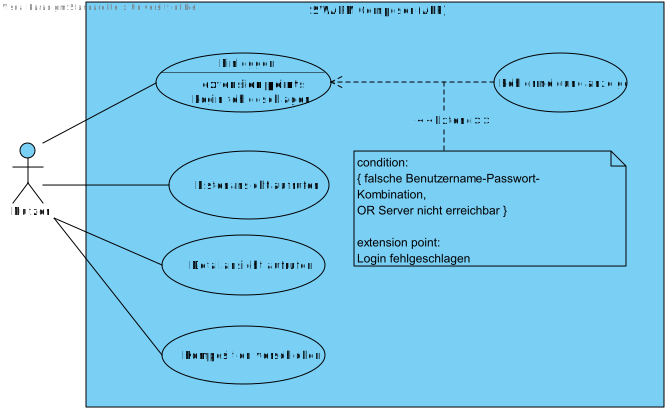
\includegraphics[width=\textwidth]{img/Produktfunktionen_app}	
	\caption{Anwendungsfalldiagramm - App}
	\label{fig:anwendungsfalldiagramm-app}
\end{figure}

\newpage

\begin{figure}[h]
	\centering
	\begin{tabularx}{\textwidth}{ X | X }
		\textbf{Anwendungsfall ID} & APP-1 \\ \hline
		\textbf{Anwendungsfallname} & Einloggen \\ \hline
		\textbf{Initiierender Akteur} & NutzerIn \\ \hline
		\textbf{Weitere Akteure} & -  \\ \hline
		\textbf{Kurzbeschreibung} & Der Nutzer loggt sich ein.  \\ \hline
		\textbf{Vorbedingungen} & Die Android-App ist geöffnet. Der Nutzer ist nicht eingeloggt.  \\ \hline
		\textbf{Nachbedingungen} & Der Nutzer ist eingeloggt.  \\ \hline
		\textbf{Ablauf} &
			\begin{enumerate}
				\item Der Nutzer gibt seinen Benutzernamen ein.
				\item Der Nutzer gibt sein Passwort ein.
				\item Der Nutzer tippt auf den Login-Button.
				\item Eine Bestätigung der erfolgreichen Anmeldung wird angezeigt.
			\end{enumerate} \\ \hline
		\textbf{Alternative} &
				- \\ \hline
		\textbf{Ausnahme} &
				\begin{enumerate}
					\item Der Nutzer gibt seinen Benutzernamen ein.
					\item Der Nutzer gibt sein Passwort ein.
					\item Der Nutzer tippt auf den Login-Button.
					\item Die Anmeldung schlägt fehl und eine Fehlermeldung wird angezeigt.
				\end{enumerate}  \\ \hline
		\textbf{Benutzte Anwendungsfälle} & Fehlermeldung anzeigen \\ \hline
		\textbf{Spezielle Anforderungen} & - \\ \hline
		\textbf{Annahmen} & -
	\end{tabularx}
	\caption{Anwendungsfall APP-1}
	\label{fig:anwendungsfall-app-tabelle-APP-1}
\end{figure}

\newpage

\begin{figure}[h]
	\centering
	\begin{tabularx}{\textwidth}{ X | X }
		\textbf{Anwendungsfall ID} & APP-2 \\ \hline
		\textbf{Anwendungsfallname} & Listenansicht aufrufen \\ \hline
		\textbf{Initiierender Akteur} & NutzerIn \\ \hline
		\textbf{Weitere Akteure} & -  \\ \hline
		\textbf{Kurzbeschreibung} & Dem Nutzer wird eine Liste von vorhandenen Kompositionen angezeigt.  \\ \hline
		\textbf{Vorbedingungen} & Die App ist geöffnet.  \\ \hline
		\textbf{Nachbedingungen} & Dem Nutzer wird eine Liste von vorhandenen Kompositionen angezeigt.  \\ \hline
		\textbf{Ablauf} &
		\begin{enumerate}
			\item Die für den Nutzer sichtbaren Kompositionen werden vom Server abgerufen.
			\item Die Daten werden als Liste angezeigt.
		\end{enumerate} \\ \hline
		\textbf{Alternative} &
		\begin{enumerate}
			\item Der Nutzer kehrt zur Listenansicht zurück.
			\item Ihm wird eine Liste der für ihn sichtbaren Kompositionen angezeigt.
		\end{enumerate}  \\ \hline
		\textbf{Ausnahme} &
		-  \\ \hline
		\textbf{Benutzte Anwendungsfälle} & - \\ \hline
		\textbf{Spezielle Anforderungen} & - \\ \hline
		\textbf{Annahmen} & -
	\end{tabularx}
	\caption{Anwendungsfall APP-2}
	\label{fig:anwendungsfall-app-tabelle-APP-2}
\end{figure}

\newpage

\begin{figure}[h]
	\centering
	\begin{tabularx}{\textwidth}{ X | X }
		\textbf{Anwendungsfall ID} & APP-3 \\ \hline
		\textbf{Anwendungsfallname} & Detailansicht aufrufen \\ \hline
		\textbf{Initiierender Akteur} & NutzerIn \\ \hline
		\textbf{Weitere Akteure} & -  \\ \hline
		\textbf{Kurzbeschreibung} & Der Nutzer ruft die Detailansicht einer Komposition auf.  \\ \hline
		\textbf{Vorbedingungen} & Der Nutzer hat die Listenansicht aufgerufen.  \\ \hline
		\textbf{Nachbedingungen} & Dem Nutzer wird die Detailansicht einer Komposition gezeigt.  \\ \hline
		\textbf{Ablauf} &
		\begin{enumerate}
			\item Der Nutzer wählt in der Listenansicht eine Komposition aus.
			\item Dem Nutzer werden die Details der ausgewählten Komposition angezeigt.
		\end{enumerate} \\ \hline
		\textbf{Alternative} &
		-  \\ \hline
		\textbf{Ausnahme} &
		- \\ \hline
		\textbf{Benutzte Anwendungsfälle} & - \\ \hline
		\textbf{Spezielle Anforderungen} & - \\ \hline
		\textbf{Annahmen} & -
	\end{tabularx}
	\caption{Anwendungsfall APP-3}
	\label{fig:anwendungsfall-app-tabelle-APP-3}
\end{figure}

\newpage

\begin{figure}[h]
	\centering
	\begin{tabularx}{\textwidth}{ X | X }
		\textbf{Anwendungsfall ID} & APP-4 \\ \hline
		\textbf{Anwendungsfallname} & Komposition verschicken \\ \hline
		\textbf{Initiierender Akteur} & Nutzer \\ \hline
		\textbf{Weitere Akteure} & -  \\ \hline
		\textbf{Kurzbeschreibung} & Der Nutzer verschickt eine Komposition.  \\ \hline
		\textbf{Vorbedingungen} & Der Nutzer hat in der Listenansicht eine Komposition ausgewählt und die Detailansicht aufgerufen.  \\ \hline
		\textbf{Nachbedingungen} & Die Komposition wird verschickt.  \\ \hline
		\textbf{Ablauf} &
		\begin{enumerate}
			\item Dem Nutzer wird eine Komposition in der Detailansicht angezeigt.
			\item Der Nutzer tippt auf den Verschicken-Button.
			\item Eine Datei im PDF-Format wird erstellt.
			\item Der Nutzer bestätigt den Versand.
		\end{enumerate} \\ \hline
		\textbf{Alternative} &
		-  \\ \hline
		\textbf{Ausnahme} &
		- \\ \hline
		\textbf{Benutzte Anwendungsfälle} & - \\ \hline
		\textbf{Spezielle Anforderungen} & - \\ \hline
		\textbf{Annahmen} & -
	\end{tabularx}
	\caption{Anwendungsfall APP-4}
	\label{fig:anwendungsfall-app-tabelle-APP-4}
\end{figure}

\newpage

%%%%%%%%%%%%%%%
%% Anwendungsfall 2 %%
%%%%%%%%%%%%%%%

\section{Anwendungsfalldiagramm - Server}

\begin{figure}[h]
	\centering
	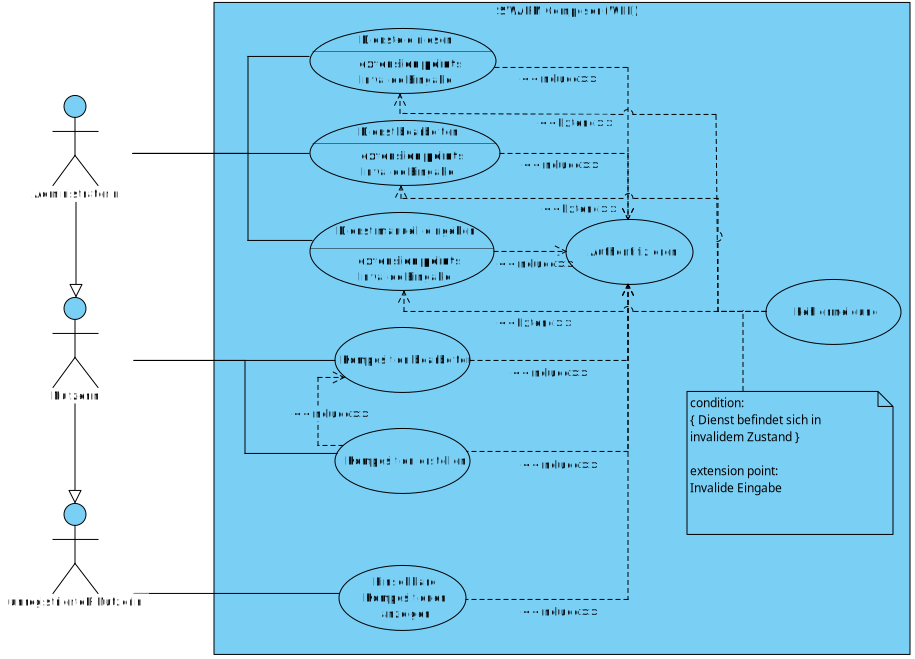
\includegraphics[width=\textwidth]{img/Produktfunktionen_web}
	\caption{Anwendungsfalldiagramm - Server}
	\label{fig:anwendungsfalldiagramm-server}
\end{figure}

\newpage

\begin{figure}[h]
	\centering
	\begin{tabularx}{\textwidth}{ X | X }
		\textbf{Anwendungsfall ID} & WEB-1 \\ \hline
		\textbf{Anwendungsfallname} & Dienst manuell einfügen \\ \hline
		\textbf{Initiierender Akteur} & AdministratorIn \\ \hline
		\textbf{Weitere Akteure} & - \\ \hline
		\textbf{Kurzbeschreibung} & Ein neuer Dienst wird in die Datenbank eingefügt. \\ \hline
		\textbf{Vorbedingungen} & AdministratorIn ist eingeloggt und befindet sich auf Administrationsseite. \\ \hline
		\textbf{Nachbedingungen} & Neuer Dienst wurde in Datenbank gespeichert. \\ \hline
		\textbf{Ablauf} &
		\begin{enumerate}
			\item [1.] [Use-Case: Authentifizieren]
			\item [2.] AdministratorIn wählt ``Dienst eingeben'' aus.
			\item [3.] AdministratorIn gibt Dienstdetails in Eingabemaske ein.
			\item [4.] AdministratorIn bestätigt die Eingabe.
			\item [5.] System akzeptiert Eingabe und speichert in Datenbank.
			\item [6.] Zurück zur Administrationsseite.
		\end{enumerate} \\ \hline
		\textbf{Alternative} & - \\ \hline
		\textbf{Ausnahme} &
		\begin{enumerate}
			\item [1.] [Use-Case: Authentifizieren]
			\item [2.] AdministratorIn wählt ``Dienst eingeben'' aus.
			\item [3.] AdministratorIn gibt Dienstdetails in Eingabemaske ein.
			\item [4.] AdministratorIn bestätigt seine Eingabe.
			\item [5.] System akzeptiert Eingabe nicht, da sie invalide ist.
			\item [6.] System zeigt Fehler an und markiert invalide Felder.
			\item [7.] Es wird in der Eingabemaske verblieben.
		\end{enumerate} \\ \hline
		\textbf{Benutzte Anwendungsfälle} & Authentifizieren \\ \hline
		\textbf{Spezielle Anforderungen} & - \\ \hline
		\textbf{Annahmen} & Die Authentifizierung ist erfolgreich.
	\end{tabularx}
	\caption{Anwendungsfall WEB-1}
	\label{fig:anwendungsfall-server-tabelle-web-1}
\end{figure}

\begin{figure}[h]
	\centering
	\begin{tabularx}{\textwidth}{ X | X }
		\textbf{Anwendungsfall ID} & WEB-2 \\ \hline
		\textbf{Anwendungsfallname} & Dienste einlesen \\ \hline
		\textbf{Initiierender Akteur} & AdministratorIn \\ \hline
		\textbf{Weitere Akteure} & - \\ \hline
		\textbf{Kurzbeschreibung} & Ein oder mehrere Dienste werden über eine JSON Datei eingelesen, die sich lokal auf einem Nutzerrechner befindet. \\ \hline
		\textbf{Vorbedingungen} & AdministratorIn ist eingeloggt und befindet sich auf Administrationsseite. \\ \hline
		\textbf{Nachbedingungen} & Neue Dienste wurden der Datenbank hinzugefügt. \\ \hline
		\textbf{Ablauf} &
		\begin{enumerate}
			\item [1.] [Use-Case: Authentifizieren]
			\item [2.] AdministratorIn wählt ``Dienste einlesen'' aus.
			\item [3.] AdministratorIn wählt die hochzuladene JSON Datei aus dem sich öffnendem Dateibrowser vom lokalen Rechner aus.
			\item [4.] Eingelesene Daten werden vom System akzeptiert und aufgelistet.
			\item [5.] AdministratorIn speichert.
			\item [6.] Dienste werden in Datenbank gespeichert.
			\item [7.] Es erscheint die Administrationsseite.
		\end{enumerate} \\ \hline
		\textbf{Alternative} & - \\ \hline
		\textbf{Ausnahme} &
		\begin{enumerate}
			\item [1.]  [Use-Case: Authentifizieren]
			\item [2.]  AdministratorIn wählt ``Dienste einlesen'' aus.
			\item [3.]  AdministratorIn wählt hochzuladene JSON Datei aus dem sich öffnenden Dateibrowser vom lokalen Rechner aus.
			\item [4.]  System erkennt Fehler in der JSON Datei und gibt einen Fehler aus.
			\item [5.]  Administrator bleibt auf der Administrationseite.
		\end{enumerate}  \\ \hline
		\textbf{Benutzte Anwendungsfälle} & Authentifizieren \\ \hline
		\textbf{Spezielle Anforderungen} & - \\ \hline
		\textbf{Annahmen} & Die Authentifizierung ist erfolgreich.
	\end{tabularx}
	\caption{Anwendungsfall WEB-2}
	\label{fig:anwendungsfall-server-tabelle-web-2}
\end{figure}

\begin{figure}[h]
	\centering
	\begin{tabularx}{\textwidth}{ X | X }
		\textbf{Anwendungsfall ID} & WEB-3 \\ \hline
		\textbf{Anwendungsfallname} & Dienst bearbeiten \\ \hline
		\textbf{Initiierender Akteur} & AdministratorIn \\ \hline
		\textbf{Weitere Akteure} & - \\ \hline
		\textbf{Kurzbeschreibung} & Felder eines existierenden Dienstes werden bearbeitet. \\ \hline
		\textbf{Vorbedingungen} & AdministratorIn ist eingeloggt und befindet sich auf Administrationsseite. \\ \hline
		\textbf{Nachbedingungen} & Vorgenommene Änderungen am Dienst wurden in Datenbank übernommen. \\ \hline
		\textbf{Ablauf} &
		\begin{enumerate}
			\item [1.] [Use-Case: Authentifizieren]
			\item [2.] AdministratorIn wählt Dienst aus Liste von vorhandenen Diensten aus.
			\item [3.] AdministratorIn wählt ``Bearbeiten''.
			\item [4.] AdministratorIn führt Änderungen in Eingabemaske durch.
			\item [5.] AdministratorIn bestätigt die Eingabe.
			\item [6.] System akzeptiert die Änderung und speichert diese in der Datenbank.
		\end{enumerate} \\ \hline
		\textbf{Alternative} & - \\ \hline
		\textbf{Ausnahme} &
		\begin{enumerate}
			\item [1.] [Use-Case: Authentifizieren]
			\item [2.] AdministratorIn wählt Dienst aus Liste von vorhandenen Diensten aus.
			\item [3.] AdministratorIn wählt ``Bearbeiten''.
			\item [4.] AdministratorIn tätigt eine invalide Eingabe.
			\item [5.] AdministratorIn bestätigt die Eingabe.
			\item [6.] System erkennt Fehler und zeigt eine Fehlermeldung an.
			\item [6.] AdministratorIn bleibt auf der Administrationsseite.
		\end{enumerate}  \\ \hline
		\textbf{Benutzte Anwendungsfälle} & Authentifizieren \\ \hline
		\textbf{Spezielle Anforderungen} & - \\ \hline
		\textbf{Annahmen} & Die Authentifizierung ist erfolgreich.
	\end{tabularx}
	\caption{Anwendungsfall WEB-3}
	\label{fig:anwendungsfall-server-tabelle-web-3}
\end{figure}

\begin{figure}[h]
	\centering
	\begin{tabularx}{\textwidth}{ X | X }
		\textbf{Anwendungsfall ID} & WEB-4 \\ \hline
		\textbf{Anwendungsfallname} & Komposition erstellen \\ \hline
		\textbf{Initiierender Akteur} & NutzerIn \\ \hline
		\textbf{Weitere Akteure} & - \\ \hline
		\textbf{Kurzbeschreibung} & Eine neue Komposition wird zum System hinzugefügt. \\ \hline
		\textbf{Vorbedingungen} & NutzerIn befindet sich auf der Übersichtsseite und ist eingeloggt.  \\ \hline
		\textbf{Nachbedingungen} & Komposition ist erstellt und NutzerIn befindet sich im Bearbeitungsmodus. \\ \hline
		\textbf{Ablauf} &
		\begin{enumerate}
			\item[1.]  [Use-Case: Authentifizieren]
			\item[2.]  NutzerIn wählt ``Komposition erstellen'' aus.
			\item[3.]  NutzerIn gibt einen Namen für die Komposition an.
			\item[4.]  NutzerIn wird weitergeleitet zum Bearbeitungsmodus.
			\item[5.] [Use-Case: Komposition bearbeiten]
		\end{enumerate} \\ \hline
		\textbf{Alternative} & - \\ \hline
		\textbf{Ausnahme} & - \\ \hline
		\textbf{Benutzte Anwendungsfälle} & WEB-5, Authentifizieren\\ \hline
		\textbf{Spezielle Anforderungen} & - \\ \hline
		\textbf{Annahmen} & Die Authentifizierung ist erfolgreich.
	\end{tabularx}
	\caption{Anwendungsfall WEB-5}
	\label{fig:anwendungsfall-server-tabelle-web-4}
\end{figure}

\begin{figure}[h]
	\centering
	\begin{tabularx}{\textwidth}{ X | X }
		\textbf{Anwendungsfall ID} & WEB-5 \\ \hline
		\textbf{Anwendungsfallname} & Komposition bearbeiten \\ \hline
		\textbf{Initiierender Akteur} & NutzerIn \\ \hline
		\textbf{Weitere Akteure} & - \\ \hline
		\textbf{Kurzbeschreibung} & NutzerIn bearbeitet Komposition. \\ \hline
		\textbf{Vorbedingungen} & NutzerIn besitzt benötigte Rechte zur Bearbeitung der Komposition und befindet sich auf der Übersichtsseite. \\ \hline
		\textbf{Nachbedingungen} & NutzerIn befindet sich im Bearbeitungsmodus. \\ \hline
		\textbf{Ablauf} &
		\begin{enumerate}
			\item[1.] [Use-Case: Authentifizieren]
			\item[2.] NutzerIn wählt ``Komposition bearbeiten'' aus.
			\item[3.] NutzerIn wird in den Bearbeitungsmodus versetzt.
		\end{enumerate} \\ \hline
		\textbf{Alternative} & - \\ \hline
		\textbf{Ausnahme} & - \\ \hline
		\textbf{Benutzte Anwendungsfälle} & Authentifizieren \\ \hline
		\textbf{Spezielle Anforderungen} & - \\ \hline
		\textbf{Annahmen} & Es werden nur Komposition gezeigt für die der NutzerIn die benötigten Rechte besitzt.
                  Der Bearbeitungsbutton ist ausgegraut, falls die Bearbeitungsrechte nicht vorhanden sind. Die Authentifizierung war erfolgreich.
	\end{tabularx}
	\caption{Anwendungsfall WEB-5}
	\label{fig:anwendungsfall-server-tabelle-web-5}
\end{figure}

\begin{figure}[h]
	\centering
	\begin{tabularx}{\textwidth}{ X | X }
		\textbf{Anwendungsfall ID} & WEB-6 \\ \hline
		\textbf{Anwendungsfallname} & Einsehbare Komposition anzeigen \\ \hline
		\textbf{Initiierender Akteur} & unregistrierteR NutzerIn oder NutzerIn\\ \hline
		\textbf{Weitere Akteure} & - \\ \hline
		\textbf{Kurzbeschreibung} & (UnregistrierteR) NutzerIn  lässt sich eine Komposition anzeigen. \\ \hline
		\textbf{Vorbedingungen} & (UnregistrierteR) NutzerIn befindet sich auf der Übersichtsseite. \\ \hline
		\textbf{Nachbedingungen} & (UregistrierteR) NutzerIn wird die Komposition angezeigt. \\ \hline
		\textbf{Ablauf} &
		\begin{enumerate}
			\item[1.] [Use-Case: Authentifizieren]
			\item[2.] (UnregistrierteR) NutzerIn wählt die anzuzeigende Komposition aus.
			\item[3.] (UnregistrierteR) NutzerIn wird die Komposition angezeigt.
		\end{enumerate} \\ \hline
		\textbf{Alternative} & - \\ \hline
		\textbf{Ausnahme} & - \\ \hline
		\textbf{Benutzte Anwendungsfälle} & Authentifizieren \\ \hline
		\textbf{Spezielle Anforderungen} & - \\ \hline
		\textbf{Annahmen} & Es werden nur Kompositionen gezeigt, für die der (unregistrierteR) NutzerIn die benötigten Rechte besitzt. Die Authentifizierung war erfolgreich.
	\end{tabularx}
	\caption{Anwendungsfall WEB-6}
	\label{fig:anwendungsfall-server-tabelle-web-6}
\end{figure}